\section{Relaxed consistency for concurrent sketches}
\label{fc-sec:concurrentSketches}

Previous work by Alistarh et al.~\cite{alistarh2018distributionally} has presented a formalization for a randomized relaxation of an object.
The main idea is to have the parallel execution approximately simulate the object’s correct sequential behavior, with some provided error distribution.
In their framework, one considers the parallel algorithm and bounds the probability that it induces a large error
 relative to the deterministic sequential specification.
This approach is not suitable for our analysis, since the sequential object we parallelize (namely the sketch) is
itself randomized. Thus, there are two sources of error: (1) the approximation error in the sequential sketch and
(2) the additional error induced by the parallelization. For the former, we wish to leverage the
existing literature on analysis of sequential sketches. To bound the latter, we use a different
methodology: we first derandomize the sequential sketch by delegating its coin flips to an oracle,
and then analyze the relaxation of the (now) deterministic sketch. Finally, we leverage the sequential sketch
analysis to arrive at a distribution for the returned value of a query.


We adopt a variant of Henzinger et al.'s~\cite{Henzinger} {\emph{out-of-order}} relaxation,  
which generalizes quasi-linearizabilty~\cite{afek2010quasi}.
Intuitively, this relaxation allows a query to ``miss'' a bounded number of updates that precede it.
Because a sketch is order agnostic, we further allow re-ordering of the updates ``seen'' by a query.

\begin{definition}[r-relaxed history]
  A sequential history $H$ is an \emph{r-relaxation} of a sequential history $H'$,
  if $H$ is comprised of all but at most $r$ of the invocations in $H'$ and their responses,
  and each invocation in $H$ is preceded by all but at most $r$ of the invocations that precede the 
  same invocation in $H'$. 
\end{definition}

A relaxed property for an object $o$ is an extension of its sequential specification to include also
relaxed histories and thus allow more behaviors. This requires $o$ to have a sequential specification, so
we convert sketches into deterministic objects by capturing their randomness in an external oracle; 
given the oracle's output, the sketches behave deterministically.
For the $\Theta$ sketch, the oracle's output is passed as a hidden variable to $init$, where the sketch
selects the hash function. In the Quantiles sketch, a coin flip is provided with every update.

For a derandomized sketch, we refer to the set of histories arising in its sequential
executions as \emph{SeqSketch}, and use SeqSketch as its sequential specification.
We can now define our relaxed semantics:
\begin{definition}[r-relaxation]
The \emph{r-relaxation} of SeqSketch is the set of histories that have r-relaxations in SeqSketch:
  
\[ SeqSketch^r \triangleq \{H'|\exists H\in \textrm{SeqSketch s.t. H is an r-relaxation of}\ H'\}.\]

\label{fc-def:r-relaxtion}
\end{definition}

Note that our formalism slightly differs from that of~\cite{Henzinger} in that we start with a serialization $H'$ of an object’s
execution that does not meet the sequential specification and then ``fix'' it by relaxing it to a history $H$ in the sequential
specification. In other words, we relax history $H'$ by allowing up to $r$ updates to ``overtake'' every query, so the
resulting relaxation $H$ is in SeqSketch.
\begin{figure}[ht]
%\begin{wrapfigure}{r}{0.4\textwidth}
    \begin{center}
      %\vspace{-0.3in}
      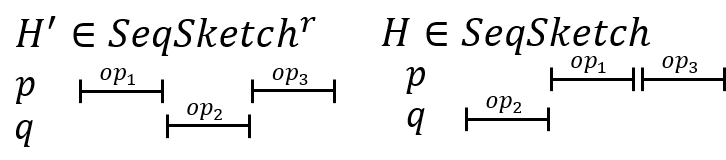
\includegraphics[width=0.5\textwidth]{graphics/fast-concurrent/relaxationExample}
      %\vspace{-0.3in}
    \end{center}
    \caption{$H$ is a 1-relaxation of $H'$.}
    \label{fc-fig:relaxationExample}
%\end{wrapfigure}
\end{figure}

An example is given in Figure~\ref{fc-fig:relaxationExample}, where $H$ is a 1-relaxation of history $H'$.
Both $H$ and $H'$ are sequential, as the operations don't overlap.
%In history $H$, $op_2$ has ``overtaken'' $op_1$ to appear first.

The impact of the $r$-relaxation on the sketch's error depends on the \emph{adversary}, which may select up to 
$r$ updates to hide from every query. There exist two adversary models:   
A \emph{weak adversary} decides which $r$ operations to omit from 
every query without observing the coin flips. 
A \emph{strong adversary} may select which updates to hide after learning 
the coin flips. Neither adversary sees the protocol's internal state, however both know the algorithm
and see the input. As the strong adversary knows the coin flips, it can then extrapolate the state; the
weak adversary, on the other hand, cannot.


